%%%%%%%%%%%%%%%%%%%%%%%%%%%%%%%%%%%%%%%%%
% Stylish Article
% LaTeX Template
% Version 2.2 (2020-10-22)
%
% This template has been downloaded from:
% http://www.LaTeXTemplates.com
%
% Original author:
% Mathias Legrand (legrand.mathias@gmail.com) 
% With extensive modifications by:
% Vel (vel@latextemplates.com)
%
% License:
% CC BY-NC-SA 3.0 (http://creativecommons.org/licenses/by-nc-sa/3.0/)
%
%%%%%%%%%%%%%%%%%%%%%%%%%%%%%%%%%%%%%%%%%

%----------------------------------------------------------------------------------------
%	PACKAGES AND OTHER DOCUMENT CONFIGURATIONS
%----------------------------------------------------------------------------------------

\documentclass[fleqn,10pt]{SelfArx} % Document font size and equations flushed left

\usepackage[english]{babel} % Specify a different language here - english by default

\usepackage{lipsum} % Required to insert dummy text. To be removed otherwise
\usepackage{bm}
\usepackage{ctex}
\usepackage{graphicx}
\usepackage{subfigure}
\usepackage{float} 
\usepackage{caption}
%----------------------------------------------------------------------------------------
%	COLUMNS
%----------------------------------------------------------------------------------------

\setlength{\columnsep}{0.55cm} % Distance between the two columns of text
\setlength{\fboxrule}{0.75pt} % Width of the border around the abstract

%----------------------------------------------------------------------------------------
%	COLORS
%----------------------------------------------------------------------------------------

\definecolor{color1}{RGB}{0,0,90} % Color of the article title and sections
\definecolor{color2}{RGB}{0,20,20} % Color of the boxes behind the abstract and headings

%----------------------------------------------------------------------------------------
%	HYPERLINKS
%----------------------------------------------------------------------------------------

\usepackage{hyperref} % Required for hyperlinks

\hypersetup{
	hidelinks,
	colorlinks,
	breaklinks=true,
	urlcolor=color2,
	citecolor=color1,
	linkcolor=color1,
	bookmarksopen=false,
	pdftitle={Title},
	pdfauthor={Author},
}

%----------------------------------------------------------------------------------------
%	ARTICLE INFORMATION
%----------------------------------------------------------------------------------------

\JournalInfo{Social network mining} % Journal information
\Archive{2021.7} % Additional notes (e.g. copyright, DOI, review/research article)

\PaperTitle{An In-depth Study of Machine Learning on Graphs} % Article title

\Authors{Lesi Chen, Junzhe Jiang, Miaopeng Yu} % Authors


\Keywords{Network analysis, Community detection, Node classification, Link prediction} % Keywords - if you don't want any simply remove all the text between the curly brackets
\newcommand{\keywordname}{Keywords} % Defines the keywords heading name

%----------------------------------------------------------------------------------------
%	ABSTRACT
%----------------------------------------------------------------------------------------

\Abstract{We finish some classic tasks of machine learning on graphs. First, we compare two representative methods(modularity-based and coding-based) to detect communities in networks. Second, we analyze and visualize the attributes of different networks(real networks and synthetic networks), and we also observe the evolution of networks. Third, we reproduce some famous models to classify the nodes in networks, including graph neural networks. Furthermore, we applied techniques for both shallow and deep graph convolution networks, outperforming the original methods. Fourth, we use graph auto-encoders for link prediction to achieve the performance of state-of-the-art, and introduce two important techniques to tackle the KL-vanishing problem in variational graph auto-encoders.} 
%----------------------------------------------------------------------------------------
\usepackage{tocvsec2}
\setcounter{tocdepth}{1}
\begin{document}
	
	\maketitle % Output the title and abstract box
	
	\tableofcontents % Output the contents section
	
	\thispagestyle{empty} % Removes page numbering from the first page
	
	%----------------------------------------------------------------------------------------
	%	ARTICLE CONTENTS
	%----------------------------------------------------------------------------------------
	
	%\section*{Introduction} % The \section*{} command stops section numbering
	
	%\addcontentsline{toc}{section}{Introduction} % Adds this section to the table of contents
	
	\section{Community detection}
	Social, technological and information systems can often be described in terms of complex networks that have a topology of interconnected nodes combining organization and randomness. 
	To study the network, a promising approach consists in decomposing the networks into sub-units or communities, which are sets of highly interconnected nodes.
	
	We use Infomap\cite{rosvall2009map} and Louvain algorithm\cite{blondel2008fast} to detect the communities below.
	
		\subsection{Infomap}
	Consider random walk, starting from a certain point j, in accordance with the probability 
	p(i|j) jump to the next point, and then jump to the next point in the same way, repeat the process. Therefore, we can get a really long sequence. Infomap detect communities in a network by minimizing the coding length of the sequence.
	\subsubsection{Two-layer coding}
	
	Infomap\cite{rosvall2009map} uses a two-layer coding rule to encode the above sequence. The two-layer coding uses a two-layer structure to divide different nodes into groups, and two types of information need to be distinguished during coding. The first is the name of the group, and the name encoding of different groups is different; the second is the node (and the exit group flag) within each group, and the name of the different node has different encoding. Note that in the coding rule the codes of nodes in different groups can be reused.
	
	Infomap's two-layer coding method connects community discovery with information coding. A good group division can lead to shorter codes. Therefore, if the group division that makes the random walk sequence length the shortest is found, then a good group division is found.
	
	
	According to Shannon's information entropy theory, the average coding length of random walk is:
	\begin{equation}
		L(M)=q_{\curvearrowright} H(Q)+\sum_{i=1}^{m} p_{\circlearrowright}^{i} H\left(P^{i}\right)
	\end{equation}
	
	Here $H(Q)$ is the frequency-weighted average length of
	codewords in the index codebook and $H(P^i)$ is frequency weighted average length of codewords in module
	code book i.
	Further, the entropy terms are weighted by the rate at which the codebooks are used. 
	With $q_{\curvearrowright}$ for the probability to exit module i, the index codebook is used at a rate $q_{\curvearrowright}=\sum_{i=1}^{m} q_{i\curvearrowright}$, the probability that the random walker switches modules on any given step. 
	With $p_\alpha$ for the probability to visit node $\alpha$, module codebook
	i is used at a rate $p_{\circlearrowright}^{i}=\sum_{\alpha \in i} p_{\alpha}+q_{i\curvearrowright }$, the fraction of time the random walk spends in module i plus the probability that it exits the module and the exit message is
	used. Now it is straightforward to express the entropies
	in $q_{\curvearrowright}$ and $p_\alpha$. For the index codebook, the entropy is
	
	\begin{equation}
		H(Q)=-\sum_{i=1}^{m} \frac{q_{i \curvearrowright}}{\sum_{j=1}^{m} q_{j \curvearrowright}} \log \left(\frac{q_{i \curvearrowright}}{\sum_{j=1}^{m} q_{j \curvearrowright}}\right)
	\end{equation}	
	
	\noindent
	and for module codebook i the entropy is
	
	\begin{small}
	\begin{equation}
		\begin{split}
			H\left(P^{i}\right)=&-\frac{q_{i\curvearrowright}}{q_{i \curvearrowright}+\sum_{\beta \in i} p_{\beta}} \log \left(\frac{q_{i \curvearrowright}}
			{q_{i \curvearrowright}+\sum_{\beta \in i} p_{\beta}}\right) \\
			&-\sum_{\alpha \in i} \frac{p_{\alpha}}{q_{i \curvearrowright}+\sum_{\beta \in i} p_{\beta}} \log \left(\frac{p_{\alpha}}{q_{i \curvearrowright}+\sum_{\beta \in i} p_{\beta}}\right)
		\end{split}
	\end{equation}
	\end{small}
	
	\subsubsection{Algorithm}
	\noindent
	Infomap takes a similar approach to PageRank to obtain the access probability of all nodes.
	
	\noindent
	With the access probability of all nodes, Infomap detects the communities in the network by:
	
	\noindent
	(1) Initialize each node as an independent community. 
	
	\noindent
	(2) Randomly sample a sequence of nodes in the graph, and try to  	assign each node to the community where the neighbor node is located in order, and assign the community where the average bit drops $L(M)$ the most to the node. 
	
	\noindent
	(3) Repeat Step2 until $L(M)$ can no longer be optimized.
	
	\subsection{Louvain}
	Louvain algorithm is another representative algorithm for community detection.   
	\subsubsection{Modularity}
	The modularity of a partition is a scalar value between $-\frac{1}{2}$ and 1 that measures the density of links inside communities as compared to links between communities. In the case of weighted networks, it is defined as
	
	\begin{equation}
		Q=\frac{1}{2 m} \sum_{i, j}\left[A_{i j}-\frac{k_{i} k_{j}}{2 m}\right] \delta\left(c_{i}, c_{j}\right)
	\end{equation}
	
	where $A_{ij}$ represents the weight of the edge between i and j, $k_i = \Sigma_{j} A_{ij}$ is the sum of the weights of the edges attached to vertex i, $c_i$ is the community to which vertex i is assigned, the $\delta$ function $\delta(u, v)$ is 1 if u = v and 0 otherwise and $m=\frac{1}{2} \sum_{i j} A_{i j}$
	
	\subsubsection{Algorithm}
	
	Our algorithm is divided into two phases that are repeated iteratively. Assume that we start with a weighted network of N nodes.
	
	\noindent
	\textbf{Part I}:
	
	\noindent
	(1)Assign a different community to each node of the network
	
	\noindent
	(2) For each node i we consider the neighbours j of i and we evaluate
	the gain of modularity that would take place by removing i from its community and by placing it in the community of j. The node i is then placed in the community for which this gain is maximum, but only if this gain is positive.
	
	\noindent
	(3) Apply (2) repeatedly and sequentially for all nodes until no further improvement can be achieved.
	
	\noindent
	\textbf{Part II}:
	
	\noindent
	Build a new network whose nodes are now the communities found during the first phase. To do so, the weights of the links between the new nodes are given by the sum of the weight of the links between nodes
	in the corresponding two communities. Once this second phase is
	completed, it is then possible to reapply the first phase of the algorithm to the resulting weighted network and to iterate.
	
	The algorithm is efficient because the gain in modularity $\Delta Q$ obtained by moving an isolated node i into a community C can easily be computed by
	
	\begin{small}
	\begin{equation}
		\begin{split}
			\Delta Q=&\left[\frac{\sum_{\text {in }}+2 k_{i, \text { in }}}{2 m}-\left(\frac{\sum_{\text {tot }}+k_{i}}{2 m}\right)^{2}\right]\\
			&-\left[\frac{\sum_{\text {in }}}{2 m}-\left(\frac{\sum_{\text {tot }}}{2 m}\right)^{2}-\left(\frac{k_{i}}{2 m}\right)^{2}\right]
		\end{split}
	\end{equation}
	\end{small}
	
	where $\Sigma_{in}$ is the sum of the weights of the links inside C, $\Sigma_{tot}$ is the sum of the weights of the links incident to nodes in C, $k_i$ is the sum of the weights of the links incident to
	node i, $k_{i,in}$ is the sum of the weights of the links from i to nodes in C and m is the sum of the weights of all the links in the network.
	
	A similar expression is used in order to evaluate the change of modularity when i is removed from its community. So we can easily evaluate the change of modularity by removing i from its community and then by moving it into a neighbouring community.
	
	\subsection{Comparison of community detection methods}
	
	The results of Infomap and Louvain algorithm when detecting communities in Facebook-combined are shown in Figure
 	\ref{cdf} and Table \ref{cdoi}.
 	
	\begin{figure}
		\centering
		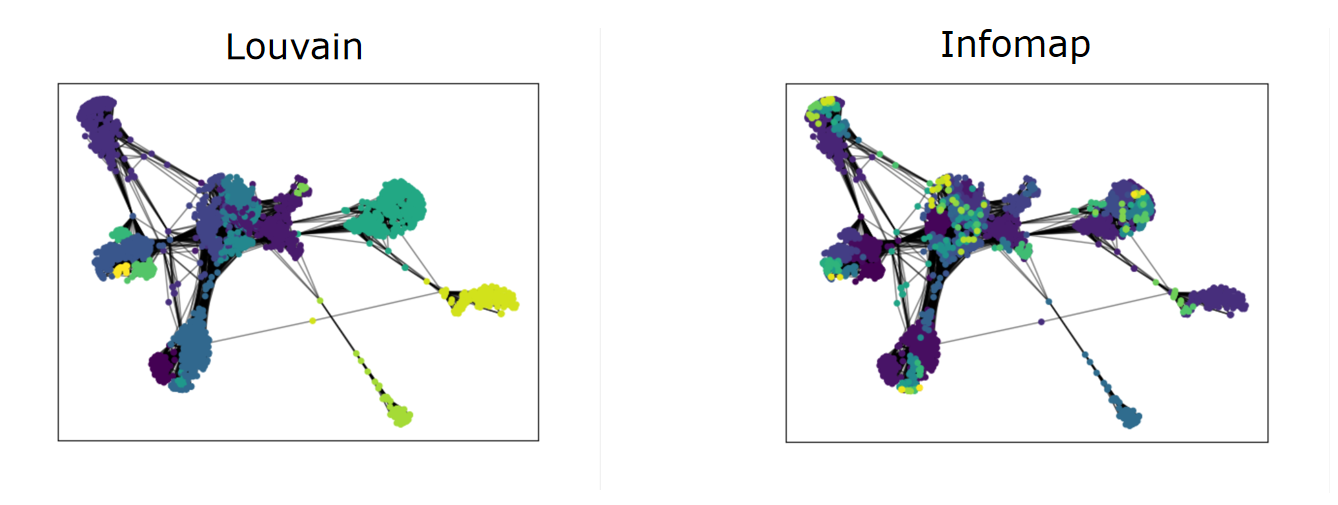
\includegraphics[width=7cm]{figure/facebook community detection.png}
		\caption{Community Detection}
		\label{cdf}
	\end{figure}
	
	\begin{table}[]
		\centering
		\begin{tabular}{lll}
			\hline
			& Louvain & Infomap \\ \hline
			number of communities & 16      & 78      \\
			modularity            & 0.83    & 0.81    \\ \hline
		\end{tabular}
		\caption{Community detection}
		\label{cdoi}
	\end{table}
	
	We can see in the Table that the modularity of communities detected by Infomap and Louvain are both relatively high. And Infomap is capable to divide more communities, indicating that it can find a more refined community structure.
	
	\section{Network analysis}
	\subsection{Centrality measurement}
	
	We select a community in facebook-combined detect by Louvain algorithm to measure the centrality of the nodes in that community. In Figure \ref{ct}, we mark the nodes with high centrality red, cyan for medium and gray for low. It can be observed that the results given by the six algorithm are similar, as is expected.
	
	\begin{figure}
		\centering
		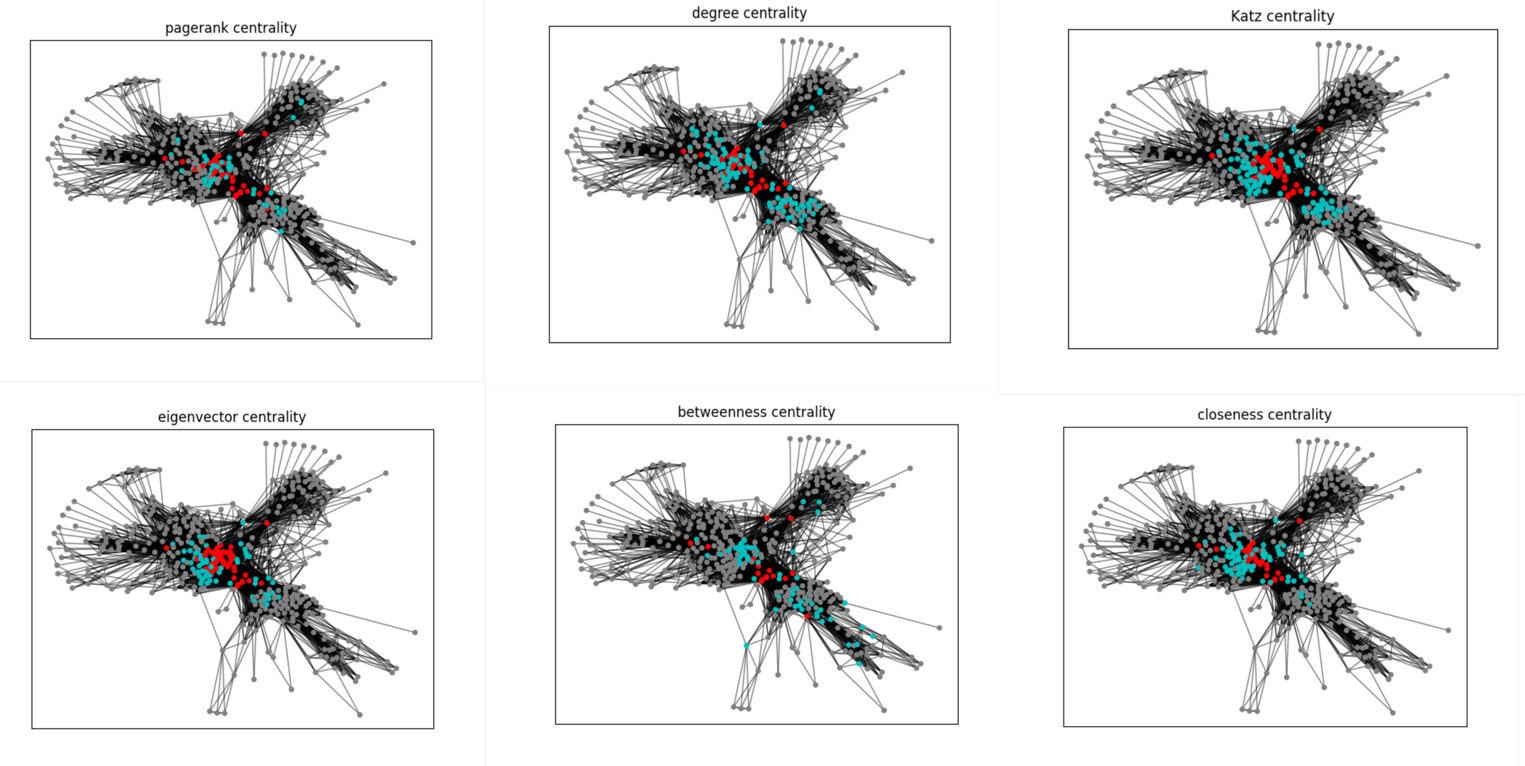
\includegraphics[width=7cm]{figure/centrality.png}
		\caption{Centrality measurement}
		\label{ct}
	\end{figure}

	\subsection{Network attribute metrics}
	We use ego-facebook and the preferential attachment graph(BA model), small world graph, random graph and complete graph for analysis in Table \ref{qtsx}, where the distance denotes the average distance between nodes and clustering denoted the clustering coefficient.
	
	\begin{table}[]
		\centering
		\begin{tabular}{lccc}
			\hline
			&distance &diameter &clustering \\ \hline
			Facebook  & 3.69& 8  & 0.606      \\
			BA  & 4.17 & 9 & 0.015   \\
			Small world    & 3.03 & 5 & 0.579   \\
			Random       & 4.42 & 9  & 0.003   \\
			Complete    & 1  & 1  & 1             \\ \hline
		\end{tabular}
		\caption{Network attribute metrics}
		\label{qtsx}
	\end{table}
	
	Also, we plotted the degree distribution of different networks in Figure \ref{dfb}. It can be seen that the real network has a smaller average distance and diameter, and a higher clustering coefficient, and the degree distribution conforms to the power-law distribution. Preferential attachment graphs and random graphs do not fit the clustering coefficients well, but degree distribution in preferential attachment graphs conforms to the power-law distribution. The small-world model can better fit the average distance, diameter and clustering coefficient, but the degree distribution does not conform to the real network at all.
	
		\begin{figure}[htbp]
		\centering  
		\subfigure 
		{
			\begin{minipage}{7cm}
				\centering  
				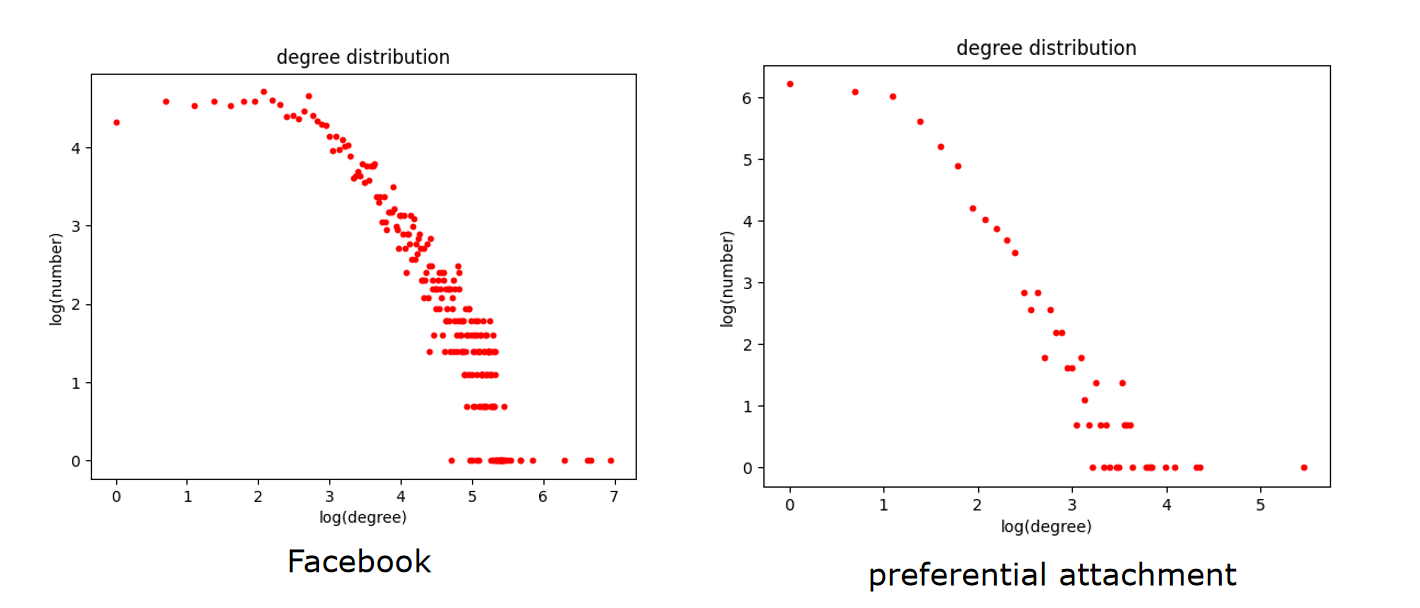
\includegraphics[width=7cm]{figure/degree1.png} 
			\end{minipage}
		}
		\quad
		\subfigure %the second subgraph
		{
			\begin{minipage}{7cm}
				\centering   
				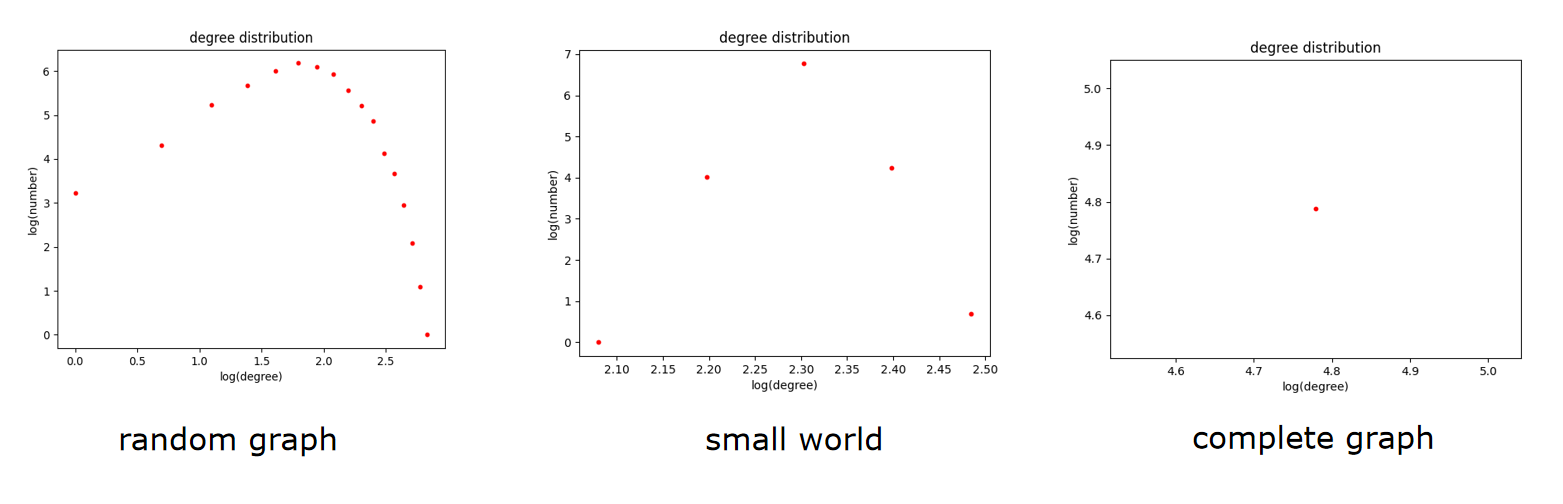
\includegraphics[width=7cm]{figure/degree2.png} 
			\end{minipage}
		}
		\caption{degree distribution}
		\label{dfb}  
	\end{figure}

	\subsection{Network evolution}
	
	First, we use ego-facebook and our link prediction model to view the evolution process. The results are shown in Table \ref{efyh}.
	
	% Please add the following required packages to your document preamble:
	% \usepackage[table,xcdraw]{xcolor}
	% If you use beamer only pass "xcolor=table" option, i.e. \documentclass[xcolor=table]{beamer}
	\begin{table}[]
		\centering
		\begin{tabular}{lccc}
			\hline
			time & distance & diameter & clustering\\ \hline
			0 & 1.95    & 2 & 0.58    \\
			1 & 1.92    & 2 & 0.29    \\
			2 & 1.88    & 2 & 0.30    \\
			3 & 1.86    & 2 & 0.32    \\
			4 & 1.83    & 2 & 0.35    \\ \hline
		\end{tabular}
		\caption{ego-facebook evolution}
		\label{efyh}
	\end{table}
	
	We can observe that the clustering coefficient decreases due to the connecting edges between non-central points. In addition, as more and more edges are linked, the network approaches to the complete graph, leading to increase of the clustering coefficient.
	
	We also use different generation probabilities to see the evolution of the random graph. The results are shown in Table \ref{randomyh} ,we set the number of nodes as 500, and we focus on the largest connected subgraph.
	
	\begin{table}[]
		\centering
		\resizebox{8cm}{15mm}{
			\begin{tabular}{lccccc}
				\hline
				time & nodes & distance & diameter & clustering & degree  \\ \hline
				0&	2&	1.00&	1&	0.0&	0.04 \\
				1&	9&	2.83&	6&	0.0&	0.56 \\
				2&	39&	6.40&	16&	0.0&	0.96 \\
				3&	497&	4.08&	8&	0.01&	4.92 \\
				4&	500&	1.90&	3&	0.1&	51.09 \\ \hline
		\end{tabular}}
		\caption{random graph evolution}
		\label{randomyh}
	\end{table}
	
	As is shown in Figure \ref{rge}, when the average degree is about 1, the average distance and diameter reach the maximum, indicating phase transition point is reached, which is also what can be proved by  theoretical analysis. 
	
	\begin{figure}
		\centering
		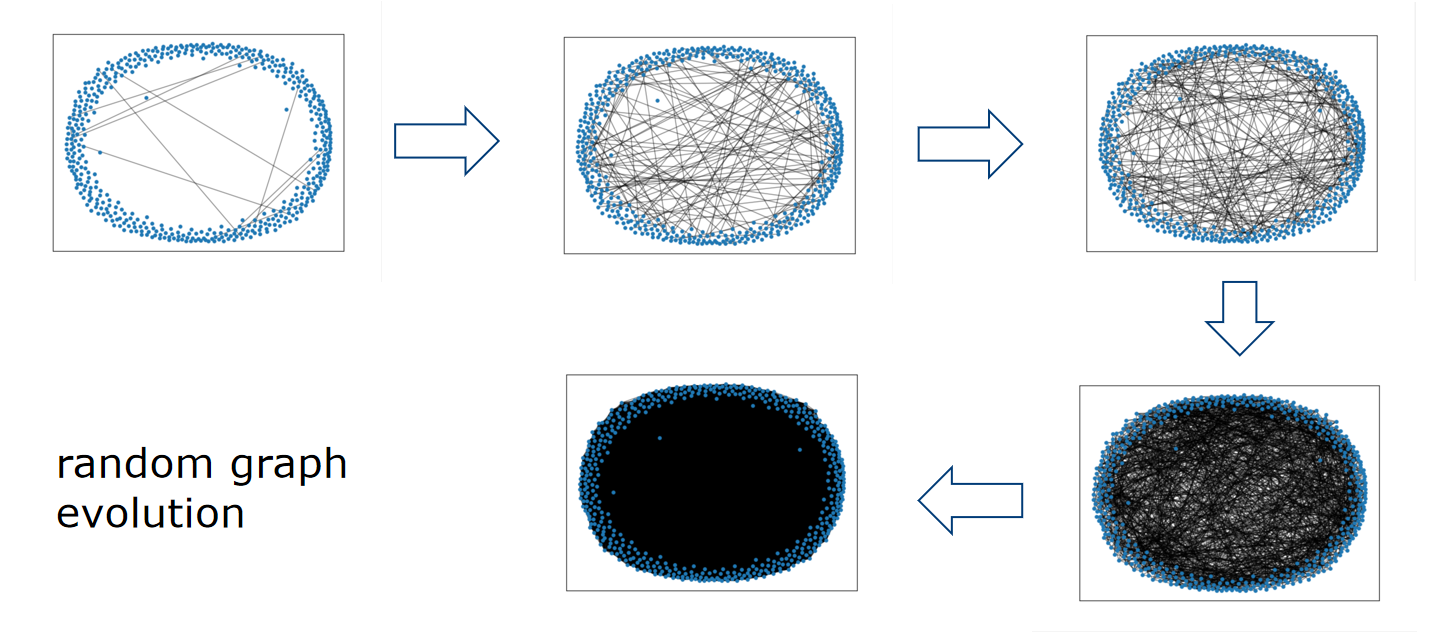
\includegraphics[width=7cm]{figure/random evolution.png}
		\caption{random graph evolution}
		\label{rge}
	\end{figure}

\section{Node classification}
%\label{section4}

\subsection{Label Propagation}

Label Propagation(LP)\cite{zhuѓ2002learning} is a simple learning-free algorithm for node classification. We first try LP on Cora, and found out that such a simple iterative algorithm can have an unexpected expressive power on Cora, achieving an accuracy of 71.30\%. The reason is that in a citation network, papers with the same class tends to cite one another, making up academic circles.

As a simple algorithm, the drawbacks of LP are obvious. First, The outcome will be unstable because a different update sequence may lead to a different classification. Second, and more importantly, without any learnable parameters, LP is less powerful than most machine learning methods.

However, we still regard LP as an important baseline for it discovers the similarity of neighbors, which is a basic idea of all the following methods we use.

\subsection{Node2Vec}
Node2Vec\cite{grover2016node2vec} is a node embedding algorithm that computes a vector representation of a node based on random walks in the graph. 
After learning the node embedding by Node2Vec, we use some classic machine learning method(eg. SVM, random forest, logistic regression) to get the prediction of the label of each node. As a semi-supervised multi-class classification task, we evaluate the cross-entropy error over all labeled examples.

We get the best accuracy using SVM (75.20\%) for learning the mapping from the hidden embedding given by Node2Vec to the node labels. As a learning method, Node2Vec outperforms LP much. However, the performance of Node2Vec is still not satisfying. We believed it is mainly because the two following reasons. First, the embedding learned by Node2Vec is 
not expressive enough as proved in \cite{levy2014neural,hamilton2017inductive}, the embedding has a rotation invariance in the hidden space, which is not required for the model to learn. Second, since the whole procedure is not learned end-to-end, the parameters of Node2Vec and SVM may not complement each other well. 

\subsection{Graph Neural Networks}
We utilize Graph Neural Networks (GNNs) for better performance. First, we investigate some representative baselines of GNNs, such as GCN\cite{chen2020simple}, GraphSAGE\cite{hamilton2017inductive} and GAT\cite{velivckovic2017graph}.

Deeply thankful to pytorch geometric, a great framework of GNNs, with the help of which, we finished all the experiments of GNNs. 

\subsubsection{Graph Convolutional Networks}
Graph Convolution Networks (GCN)\cite{chen2020simple} is a scalable approach for semi-supervised learning on graph-structure data. The convolutional architecture in GCN is motivated by a localized first-order approximation of spectral graph convolution. And the model scales only linearly  in the number of graph edges and learns hidden layer representation. 

\subsubsection{GraphSAGE}
GraphSAGE\cite{hamilton2017inductive} is an inductive algorithm for computing node embeddings. GraphSAGE uses node feature information to generate node embeddings on unseen nodes or graphs. Instead of training individual embeddings for each node, the algorithm learns a function that generates embeddings by sampling and aggregating features from a node$'$s local neighborhood.

\subsubsection{Graph Attention Networks}
Graph attention networks (GATs)\cite{velivckovic2017graph} leverages self-attentional 
layers to address the shortcomings of prior methods based on graph 
convolutions or their approximations. By stacking layers in which  nodes are able to attend over their neighborhoods’ features, GAT enables 
(implicitly) specifying different weights to different nodes in a 
neighborhood, without requiring any kind of costly matrix operation 
or depending on knowing the graph structure upfront. 

\subsection{Comparison of classic GNNs}
In the comparison of GNNs, we set train the models for 200 epochs on Cora dataset, using SGD with the learning rate of 0.01 and weight decay of 5e-4, as a general setup. The results are shown in Table \ref{node-cls}.

As transductive models, GCN (81.80\%) and GAT (81.19\%) get much better results than the inductive model GraphSAGE (79.60\%), since the node classification task in this project is also a transductive learning task. With attention mechanisms, GAT outperforms GCN little with more computation complexity, more hyperparameters and larger convergence rate. Plus, GCN has a rigorous theoretical derivation which is not provided by GAT.

For comprehensive consideration, we choose GCN as our basic model and also implement it inherited from the MessagePassing class in pytorch geometric.

\begin{table}
	\centering
	\begin{tabular}{ll}
		\toprule
		Method &    Accuracy (\%) \\
		\midrule
		LP & 71.30  \\
		Node2Vec  & 75.20\\
		GCN & 81.10 \\
		GraphSAGE & 79.60 \\
		GAT & 81.19 \\
		\bottomrule
	\end{tabular}
\caption{Node classification on Cora}
\label{node-cls}
\end{table}

\section{Improvement for node classification}
\subsection{Better optimizers}

As mentioned above, we use SGD for training GNNs. In this section, we try to use some more advanced optimizers for improvement, including 
Kronecker-factored approximate curvature(K-FAC)\cite{martens2015optimizing} and Sharpness-aware minimization(SAM)\cite{foret2020sharpness} .

In our experiment, K-FAC bring less improvement, while SAM is indeed helpful. It is worth noting that we, for the first time, try to use  SAM, to train GNNs. We successfully verified that SAM can not only play an important role in  training convolution neural networks(CNNs) in computer vision, but SAM also works in training graph neural networks. 

\subsubsection{Kronecker-factored approximate curvature}
Kronecker-factored approximate curvature (K-FAC) is a second-order optimization method based on natural gradient descent, and it effectively approximates the Fisher information 
matrix. And the approximation has the form of what is known as a Khatri-Rao product in multivariate statistics.

\subsubsection{Sharpness-Aware Minimization}
Optimizing only training loss value as is commonly done, can easily 
lead to suboptimal model quality. And the procedure Sharpness-Aware 
Minimization(SAM)\cite{foret2020sharpness}, motivated by prior work connecting geometry of 
the loss landscape and generalization, an effective procedure 
simultaneously minimizing loss value and loss sharpness, and this 
formulation results in a min-max optimization problem on which gradient 
descent can be performed efficiently:

For any $\rho > 0$, with high probability over training set $\mathcal{S}$ 
generated from distribution $\mathcal{D}$,
\begin{small}
\begin{equation}
	L_{\mathcal{D}}(w) \leq \max_{\|\epsilon \|_{2} \leq \rho} L_{\mathcal{S}}(w + \epsilon) + h(\|w\|_{2}^{2}/ \rho^{2})
\end{equation}
\end{small}
where $h: \mathbb{R}_{+}\rightarrow \mathbb{R}_{+}$ is a strictly increasing function (under some technical conditions on $L_{\mathcal{D}}(w)$). And inspired by the terms from the bound, the author of SAM proposed to select parameter values by 
solving the following SAM problem:
\begin{small}
	\begin{equation}
		\min_{w} L_{\mathcal{S}}^{SAM}(w) + \lambda \|w\|_{2}^{2}  
	\end{equation}
	where $L_{\mathcal{S}}^{SAM}(w) = \max_{\|\epsilon\|_{p} \leq \rho} L_{\mathcal{S}}(w+\epsilon)$, 
	$\rho \geq 0$ is a hyperparameter. In our experiment, we set $\rho$ as 0.5.
\end{small}

Note that SAM is based on other optimizers(eg. SGD, Adam) with approximate to minimize this problem. In our experiment, we use SGD as our base optimizer, with the same learning rate and weight decay we set in training vanilla GCN. Our results are in Table \ref{cmp=node-cls}.

\begin{table}
	\centering
	\resizebox{5cm}{1.5cm}{
	\begin{tabular}{lcc}
		\toprule
		Method &  Optimizer &  Accuracy(\%) \\
		\midrule
		GCN  & SGD & 81.1 \\
		GAT  & SGD &81.9 \\
		GCN & K-FAC    & 81.7\\
		GCN & SAM    & 82.1 \\
		GAT & SAM & 82.3 \\
		\bottomrule
	\end{tabular}}
\caption{Node classification with different optimizers}
\label{cmp=node-cls}
\end{table}

\subsection{Correct and smooth}
Correct and Smooth (C\&S)\cite{huang2020combining} is a graph representation learning method based on iteration. C\&S combines LP\cite{zhuѓ2002learning} into simple models(eg. MLP), with a understanding of the essence of GNNs, which can be summarized as correct and smooth.

C\&S first uses "error correlation" to correct errors by spread residual errors in training data to test data. And then it uses "prediction correlation" to smooths the predictions on the test data.The residuals $E$ corresponding to training nodes are zero only when 
the base predictor makes a perfect prediction:
\begin{small}
\begin{equation}
	\hat{E} = \arg \min_{W \in \mathbb{R}^{n\times c}} trace \left(W^{\top} (I-S)W\right) + \mu \|W-E\|_{F}^{2}
\end{equation}
\end{small}
and the solution can be obtained via iteration:
\begin{small}
\begin{equation}
	E^{(t+1)} = (1-\alpha)E + \alpha SE^{(t)}  
\end{equation}
\end{small}
where $\alpha = 1/(1+\mu)$ and $E^{(0)} = E$, which converges rapidly to $\hat{E}$.

After the correct iteration mentioned above, C\&S uses a smooth iteration, encouraging smoothness over the distribution over labels by another label propagation. 
C\&S iterate
$G^{(t+1)} = (1-\alpha)G + \alpha SG^{(t)}$ with $G^{(0)} = G$ until converge to 
give the final prediction $\hat{Y}$, where $G$ is out best guess of the model, and 
$G_{L_{t}} = Y_{l_{t}}$, $G_{L_{v}, U} = Z_{L_{v}, U}^{(r)}$. $Y$ is the label matrix, 
and Z is the base prediction.

Note that C\&S can be regarded as a post-processing method to improve the prediction given by any base predictor. We first reproduced the experiment in \cite{huang2020combining}, which used MLP as the base predictor. And we found that C\&S gives more than 20\% improvement to MLP. In addition, if we use GCN as the base predictor, GCN+C\&S can outperform with a improvement of approximate 1\%, with 5 iterations for correcting and 5 iterations for smoothing. Our results are shown in Table \ref{node-cls-cs}. 

\begin{table}
	\centering
	\resizebox{5cm}{1.5cm}{
	\begin{tabular}{lccc}
		\toprule
		Method & C\&S & SAM & Accuracy(\%) \\
		\midrule
		MLP    & & & 51.8     \\
		MLP  & $\surd$ &   & 72.9  \\
		GCN  & &  & 81.80 \\
		GCN  & $\surd$ &    & 82.1  \\
		GCN  & $\surd$ &  $\surd$ & 83.0  \\
		\bottomrule
	\end{tabular}}
	\caption{Node classification with shallow GCNs}
	\label{node-cls-cs}
\end{table}


\subsection{Deep GCN}

According to the over-smoothing effect, deepen the GNN endlessly may not be a wise  choice. In the meanwhile, six degrees of separation also points out that we do not need GNN with so many layers.However, the great success of deep learning heavily depends on the application of deeper neural networks. Therefore, proposing new methods to handle the paradox may be the key to improve GNNs. Recent works such as DropEdge\cite{rong2019dropedge}, Jump Knowledge Network (JKNet) \cite{xu2018representation} make efforts to solve this problem.

DropEdge\cite{rong2019dropedge} drops some edges randomly while training. And it is proved that DropEdge can reduce 
the issue of over-fitting and over-smoothing by regarding GNN as a dynamic system as in \cite{oono2019asymptotic}, significantly improving the performance of deep GCN.

JKNet\cite{xu2018representation} uses a jumping knowledge operation, which is similar to the dense connection in DenseNet\cite{huang2017densely} 
In the last layer of JKNet, each node will combine the output in each layer. And there are 3 methods proposed by JKNet to merge these nodes: concatenation, max-pooling, and LSTM-attention. In our experiment, we simply use the concatenation for GCN recommended by \cite{xu2018representation}.

In our experiment, we found that the use of Jump Knowledge and DropEdge can supplement each other. To avoid over-fitting effect of deep GCNs ,w e add the Dropout layer between GCN layers. Interestingly, using 
Jump Knowledge and DropEdge can make the Dropout rate up to 0.9, which is impossible for vanilla GCN.

Table \ref{deep-gcn} shows the results of deep GCNs. We did our experiments with GCN of 2,4,8 layers (GCN2,GCN4,\\GCN8). From the table, we can see the over-smoothing effect of vanilla GCN, and the improvement brought by JumpKnowledge and DropEdge.Adding all the techniques, deep GCNs (GCN4, GCN8) overcome over-smoothing and outperform shallow GCN(GCN2).

\begin{table}
	\centering
	\resizebox{5cm}{2cm}{
	\begin{tabular}{cccc}
		\toprule
		Method &  DropEdge & JK &Accuracy(\%) \\
		\midrule
		GCN2   & & & 81.1     \\
		GCN2   & $\surd$ & & 82.4  \\
		GCN4   & & & 62.5     \\
		GCN4   & $\surd$ & & 69.5  \\
		GCN4    & $\surd$ & $\surd$ & 82.9 \\
		GCN8   & & & 56.4     \\
		GCN8   & $\surd$ & & 65.2  \\
		GCN8    & $\surd$ & $\surd$ & 82.8 \\
		\bottomrule
	\end{tabular}}
	\caption{Node classification with deep GCNs}
	\label{deep-gcn}
\end{table}

\subsection{Go deeper with GCNII}
Graph convolutional network via initial residual and 
identity mapping (GCNII) \cite{chen2020simple}is an extension of the vanilla GCN model with two  simple yet effective techniques: Initial residual and Identity mapping. And these two techniques effectively relieve the problem of over-smoothing and improve the performance of GCNII consistently as we increase its network depth. With GCNII, we can go far deeper. The network in GCNII has a depth of 64, which is 8 times of GCN8 we implemented above.

With deeper network structure, the classification accuracy of GCNII can reach 85.5\%. In addition, with SAM as the optimizer instead of SGD, GCNII can reach an accuracy of 86.5\%, verifying the effectiveness of SAM again.In our experiment, we found that despite the upper bound of GCNII, the accuracy of GCNII fluctuates between 83\% and 86\%. Therefore, future work of GCNII may focus on enhancing the stability such a deep GNN as GCNII.

\section{Link prediction}
%\label{section5}
Link prediction can be regarded as a binary classification problem, which given arbitrary two nodes, and judge if there is an edge between these two nodes. 

\subsection{Variational Graph Auto-Encoder}
Variational graph auto-encoder(VGAE)\cite{kipf2016variational} is a framework for unsupervised learning on graph 
structure based on the Variational auto-encoder (VAE), which makes use of latent variables and is capable of learning interpretable latent representations for graphs.

The architecture of VGAE consists of an inference model and a generative model. In our experiment, we use a simple inference model parameterized by a two-layer GCN and a generative prediction given by inner product between latent variables. When training, VGAE optimize the Variational lower bound:
\begin{small}
\begin{equation}
	\mathcal{L} = \mathbb{E}_{q\left(\textbf{Z} | \textbf{X}, \textbf{A} \right)} [\log p\left(\textbf{A} | \textbf{Z} \right)] - \text{KL}[q\left(\textbf{Z} | \textbf{X}, \textbf{A} \right) \parallel  p\left(\textbf{Z} \right)],
\end{equation}
\end{small}
where $\text{KL}[q(\cdot) \parallel p(\cdot)]$ is the Kullback-Leibler divergence between 
$q(\cdot)$ and $p(\cdot)$.

\subsection{Graph Auto-Encoder}
Graph auto-encoder (GAE) is a non-probabilistic variant of the VGAE model. The loss function of GAE is defined by the
reconstruction error of the graph data:
\begin{small}
\begin{equation}
	\mathcal{L} = \mathbb{E}_{q\left(\textbf{Z} | \left(\textbf{X}, \textbf{A} \right) \right)} 
	[\log p (\hat{\textbf{A}} | \textbf{Z} )]
\end{equation}
\end{small}
which is equal to the loss function of VGAE removing the KL term.

\section{Improvement for link prediction}
GAEs typically focus on preserving the topological structure or minimizing the reconstruction errors of graph data, but they have mostly ignored the data distribution of the latent codes from the graphs, which often results in inferior embedding in real-world graph data.

VGAEs attach more importance to the distribution of latent codes, however, in our experiments, we can not find the advantage of VGAEs against GAEs. We believe the problem may lie in the KL-vanishing problem, or posterior collapse\cite{bowman2015generating}.

To tackle this problem, Sphere-VGAE(S-VGAE) \cite{davidson2018hyperspherical,xu2018spherical} and 
Adversarial Regulated VGAE(ARVGAE)\cite{pan2018adversarially} are tried. We verified that both of them can significantly improve the performance of vanilla VGAE.

\subsection{Sphere-VGAE (S-VGAE)}
Since the posterior distributions are defined as a normal distribution, former VGAE has the issue of 
KL-vanishing problem. Sphere-VGAE (S-VGAE) \cite{davidson2018hyperspherical,xu2018spherical} address this issue by altering the normal distribution by von Mises-Fisher (vMF) distribution .

And since in S-VGAE, KL divergence only depends on fixed hyperparameter $\kappa$, and it increases monotonically with $\kappa$, as does concentration measured by cosine similarity.Therefore, by controlling the hyperparameter $\kappa$, S-VGAE makes the KL divergence has a positive lower bound. In our implement, we simply add a scalar 1 on the $\kappa$ encoded by the GCN encoder.

\subsection{Adversarial Regulated VGAE}
Adversarial Regulated VGAE(ARVGE)\cite{pan2018adversarially} is an adversarial graph embedding framework for graph data that not only make use of the distribution of nodes as in VGAE, but also introduce Generative Adversarial Networks (GANs) into GNNs.The workflow of ARVGE consists of two modules: the graph auto-encoder which is the same as VGAE and the adversarial network which serves as the adversarial regularization.

The author of ARVGE gave explanation of the success of ARVGE from the perspective of regularization. However, we regard the adversarial network as also a solution of the KL-vanishing problem. Even the KL divergence collapse to zero, the discriminator will still force the latent codes to match a prior distribution
by discriminating whether the current latent code $\textbf{z}_i \in \textbf{Z}$ comes from the encoder or from the prior distribution.

The equation for training the encoder model with Discriminator $\mathcal{D}(\textbf{Z})$ can be
written as follows:
\begin{small}
\begin{equation}
\min_{\mathcal{G}} \max_{\mathcal{D}} \mathbb{E}_{\textbf{z} \sim  p_{z}} [\log \mathcal{D}(\textbf{Z})] + \mathbb{E}_{\textbf{x} \sim p(x)} [\log (1 - \mathcal{D}(\mathcal{G}(\textbf{X}, \textbf{A})) )]
\end{equation}
\end{small}
where $\mathcal{G}(\textbf{X}, \textbf{A})$ and $\mathcal{D}(\textbf{Z})$ indicate the generator and discriminator.

\subsection{Results}
The results of these methods are shown in Table \ref{link-prediction}.
We use Adam optimizer to train our link prediction models for 600 epochs. The reason we do not use SAM is because the negative sampling in link prediction makes the deduction in SAM invalid.In VGAE and GAE we use a learning rate of 0.01, while we found the learning rate of 0.02 is better when training S-VGAE. As for ARVGE, we train the encoder with the learning rate of 0.05 and the discriminator of 0.01.

\noindent
Note that by introducing Sphere-VGAE and ARVGE, our models for link prediction achieve the state-of-the-art level.
\begin{table}
	\centering
	\resizebox{5cm}{1.5cm}{
	\begin{tabular}{lll}
		\toprule
		Method &    AUC(\%) & AP(\%) \\
		\midrule
		GAE     & 91.14    & 91.28  \\
		VGAE    & 90.56  & 91.56\\
		ARVGE    & 92.50 & 92.90 \\
		S-VGAE  & 92.88 & 93.1 \\
		\bottomrule
	\end{tabular}}
	\caption{Link prediction on Cora}
	\label{link-prediction}
\end{table}
\section{Conclusion}

\noindent
\textbf{1.}Use Louvain algorithm for high modularity and Infomap for finest community structure.

\noindent
\textbf{2.}Clustering coefficient increases when real networks \\
evolve.

\noindent
\textbf{3.}The phase transition point is reached when average degree of random graph reached 1.

\noindent
\textbf{4.}Use SAM for better performance in node classification.

\noindent
\textbf{5.}Deeper GCNs is better than shallow GCNs after tackling the over-smoothing. 

\noindent 
\textbf{6.}Tackle the KL-vanishing problem for performance improvement in VGAE.
%----------------------------------------------------------------------------------------
%	REFERENCE LIST
%----------------------------------------------------------------------------------------

\phantomsection
\bibliographystyle{unsrt}
\bibliography{sample.bib}

%----------------------------------------------------------------------------------------

\end{document}